\chapter{Sistemas de Detecção e Prevenção de Intrusão} \label{ch:idps}

Os sistemas de detecção e prevenção de intrusão (\textit{Intrusion Detection and Prevention System} - IDPS) são ferramentas de importância reconhecida pela comunidade da segurança da informação, pois elas são capazes de detectar se alguém está tentando entrar no sistema ou se algum usuário legitimo está fazendo mau uso do mesmo.

Nesse capítulo, vamos apresentar os principais conceitos relacionados a IDS e IPS, uma breve descrição do funcionamento e classificação, para melhor entendimento das ferramentas que iremos apresentar e avaliar em um ambiente de real.

\section{Definições de IDS/IPS} \label{sec:ipds-definicoes}

\textit{Intrusion Detection Systems} (IDS) ou Sistemas de Detecção de Intrusão (SDI) são ferramentas utilizadas para monitoramento de eventos que ocorrem em redes e sistemas computacionais, analisando sinais de possíveis ataques que podem levar a uma violação das politicas de segurança da organização, alertando os administradores do sistema que estes eventos estão ocorrendo \cite{nagahama2012ipsflow}. 

O \textit{Intrusion Detection Systems} (IPS) ou Sistema de Prevenção de Intrusão (SPI) possui todas as funcionalidades do IDS com uma diferença, ele é capaz de deter os incidentes, minimizando os impactos causados por sistemas comprometidos \cite{mukhopadhyay01}.

%localizar a referencia
Os IDS's são compostos basicamente por quatro componentes:
\begin{alineas}
\item \textbf{Sensor ou Agente}: responsável pelo monitoramento e analise do trafego capturado; 
\item \textbf{Base de Dados}: usado como repositório das informações de eventos detectados pelo sensor e que posteriormente serão processados;
\item \textbf{Gestor}: é o dispositivo central que recebe, analisa e gerencia as informações de eventos vindo do sensor; 
\item \textbf{Console}: é uma interface para administração e monitoramento das atividades.
\end{alineas}

\section{Tipos de Sistemas de Detecção e Prevenção de Intrusão} \label{sec:idps-tipos}

Os IDPS's são classificados de acordo com o local onde o sensor é instalado, \textit{Host Based Intrusion Detection Systems} (HIDS) e \textit{Network Based Intrusion Detection Systems} (NIDS), e a técnica utilizada para o monitoramento, baseado em assinaturas e anomalias \cite{nagahama2012ipsflow}.

\subsection{Sistemas de Detecção de Intrusão Baseados em Host (HIDS)}

Em um HIDS o sensor é instalado no \textit{host}, monitorando as informações contidas na própria máquina. Esse tipo de IDS não observa o tráfego que passa pela rede (somente o trafego que passa pela placa de rede do \textit{host}), seu uso volta-se a verificação de informações relativas aos eventos e registros de logs e sistemas de arquivos (permissão, alteração, acesso a arquivos não autorizados) \cite{nagahama2012ipsflow}.  

As vantagens do HIDS são: 

\begin{alineas}
\item Evita a execução de códigos maliciosos;
\item Bloqueia tráfego de entrada e saída contendo ataques e uso não autorizado de protocolos e programas;
\item Evita que arquivos possam ser acessados, modificados e deletados impedindo a instalação de \textit{malwares} e ataques envolvendo acesso inapropriado a arquivos;
\end{alineas}

Por outro lado, o HID possui alguns desvantagens como \cite{scarfone01}:  

\begin{alineas}
\item Difícil instalação e manutenção;
\item Interfere no desempenho do \textit{hosts};
\item Demora para identificar eventos consequentemente a resposta ao incidente terá um atraso.
\end{alineas}

\subsection{Sistemas de Detecção de Intrusão Baseados em Rede (NIDS)}

No NIDS, o sensor é instalado na rede e a interface de rede atua em um modo especial chamado ``promíscuo'', tendo a capacidade de capturar o tráfego mesmo que os pacotes não sejam destinados ao sensor. Dessa forma, o NIDS monitora e analisa todo o trafego no segmento da rede, detectando atividades maliciosas, como ataques baseados em serviço, \textit{portscans}, entre outros, além de detectar se algum usuário legítimo está fazendo mau uso da rede \cite{nagahama2012ipsflow}.

Quanto a localização o NIDS pode ser classificado como passivo ou ativo. No modo passivo (\autoref{fig_nids-ativo}), o IDS monitora copias dos pacotes da rede que passam pelo \textit{switch} ou \textit{hub} onde está conectado, ficando limitado somente a gerar notificações quando encontrado algum tráfego malicioso. 

No entanto, no modo ativo (\autoref{fig_nids-passivo}), o IDS é instalado da forma que o tráfego da rede passe através do sensor parecendo com o fluxo de dados associado com um \textit{firewall}. Dessa forma, ele é capaz de parar ataques bloqueando o fluxo malicioso. 

É necessário uma analise minuciosa na instalação de um IDS ativo pois um mal dimensionamento de \textit{hardware} pode degradar a rede, adicionando atrasos excessivos aos pacotes.

As principais vantagens do um NIDS são: 

\begin{alineas}
\item São independentes de plataformas;
\item Não interfere no desempenho do \textit{host};
\item Fácil implantação e transparente para o atacante.
\end{alineas}

Dentre as desvantagens, temos:

\begin{alineas}
\item Pode adicionar retardados aos pacotes quando instalado no modo ativo;
\item Dificuldade de tratar dados de redes de alta velocidade;
\item Trata apenas segmentos de rede;
\item Dificuldade de tratar dados criptografados.
\end{alineas}

%Devido a grande heterogeneidade de dispositivos e sistemas operacionais na rede, a utilização desse tipo de IDS torna a administração mais simples se comparados com o HIDS.

\begin{figure}[!htb]
 \label{fig_nids-arquitetura}
 \centering
 \begin{minipage}{0.4\textwidth}
  \centering
  \caption{Exemplo de arquitetura de NIDS passivo} \label{fig_nids-passivo}
  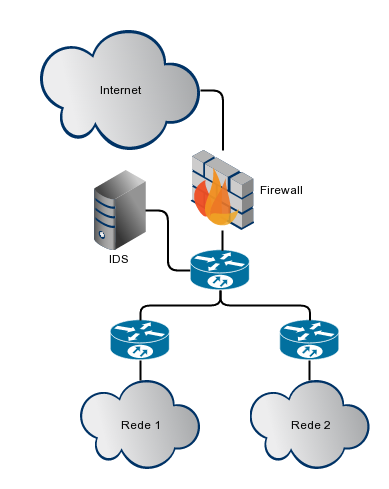
\includegraphics[scale=.55]{nids_passivo.png}
  \legend{Fonte: Autoria própria}
 \end{minipage}
 \hfill
 \begin{minipage}{0.4\textwidth}
  \centering
  \caption{Exemplo de Arquitetura de NIDS ativo} \label{fig_nids-ativo}
  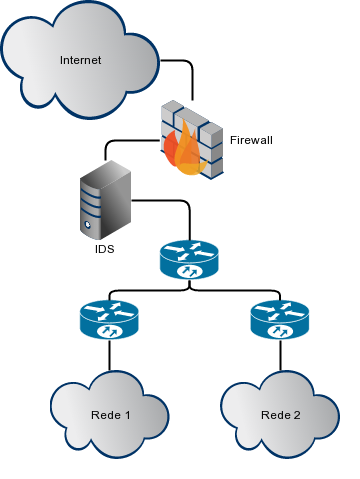
\includegraphics[scale=.55]{nids_ativo.png}
  \legend{Fonte: Autoria própria}
 \end{minipage}
\end{figure}

\subsection{Sistema de Detecção de Intrusão Distribuídos}

A função de um Sistema de Detecção de Intrusão Distribuído (SDID) é de gerencia. Os sensores (pode ser NIDS, HIDS ou a combinação de ambos), localizados remotamente, enviam, periodicamente, os alertas para um servidor central onde todas essas informações serão armazenadas, em uma base única e centralizada. Além disso, novas assinaturas de ataques podem ser enviadas para os sensores através desse servidor, dessa forma, facilitando o gerenciamento \cite{snort:andrew}.

\begin{figure}[!htb]
  \centering
  \caption{Sistema de Detecção de Intrusão Distribuído} \label{fig_dids}
  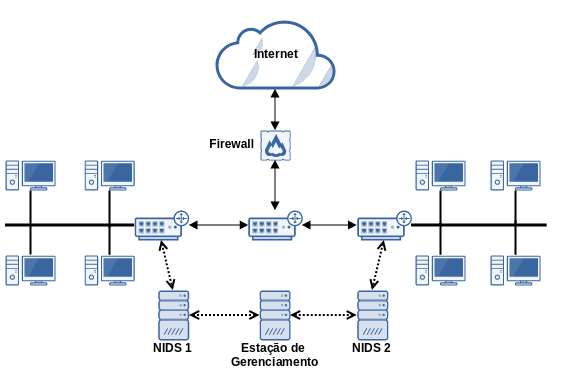
\includegraphics[scale=0.7]{dids.png}
  \legend{Fonte: Autoria própria}
\end{figure}

A \autoref{fig_dids} mostra um SDID composto por dois sensores e um estação de gerenciamento centralizado. O sensor NIDS 1 e NIDS 2 estão operando em modo \textit{promiscuos} e está monitorando segmentos de rede. É recomendando que a conexão entre os sensores e o centralizado seja feita por uma rede privada. Em caso de utilização de rede públicas, recomenda-se adicionar uma camada de segurança, como criptografia, ou VPN.

\subsection{Formas de Detecção} \label{sec:idps-formas}

Quanto a técnica de monitoramento utilizado, o IDS pode ser baseados em assinaturas ou anomalias. IDSs baseados em assinaturas compara os pacotes com uma base de assinaturas de ataques previamente conhecidos e reportados por especialistas, cada assinatura identifica um ataque \cite{nagahama2012ipsflow}.  

As vantagens de um IDS baseados em assinaturas são:

\begin{alineas}
\item Usa pouco recurso de \textif{hardware} do servidor;
\item Possui, de certa forma, um rápido processamento.
\end{alineas}

Dentre as desvantagens temos:

\begin{alineas}
\item Exige uma atualização constante da base de assinaturas;
\item Para a geração de uma base própria, a equipe precisa de um alto conhecimento técnico;
\item Possui altos índices de falsos positivos e negativos.
\end{alineas}

Os IDS baseados em anomalias, procuram determinar um comportamento normal na fase de aprendizagem do sistema computacional ou rede e sempre que existir um desvio desse padrão alertas são gerados. 

Possui a vantagem de detectar novos ataques sem necessariamente conhecer a fundo a intrusão através dos desvios de comportamento. Porém, tem como desvantagem a geração de um grande número de falsos alertas em decorrência a modificações na rede ou \textit{host} nem sempre representar um tráfego malicioso. 

\section{Principais Ferramentas de IDS} \label{sec:idps-ferramentas}

Nessa seção, será apresentado as ferramentas de IDPS. A escolha dessas ferramentas deu-se devido ser de código aberto e de livre uso, e também, por essas ferramentas não precisarem, para seu funcionamento, de um \textit{hardware} robusto.

\subsection{Snort} \label{sec:snort}

O Snort é um sistema de detecção e prevenção de intrusão de código fonte aberto escrita na linguagem de programação C. Seu primeiro \textit{release} foi lançado em 1998 e desde então passa por constantes revisões e aperfeiçoamentos, com o passar dos anos se tornou o IDS mais utilizado no mundo. Ele combina análise baseada em assinaturas e anomalias, podendo operar em três modos: \textit{sniffer}, \textit{packet logger} e de sistema de detecção de intrusão (NIDS) \cite{snort:manual}.

No modo \textit{Sniffer}, o Snort captura os pacotes e exibe as informações no console de forma continua. No modo \textit{Packet Logger}, além de capturar o tráfego, o Snort escreve essas informações em arquivos (chamados de logs) que são armazenados no disco. Por fim, o \textit{Network Intrusion Detection System} - NIDS, sendo o modo mais complexo e completo, permitindo capturar e analisar os pacotes de rede em tempo real \cite{snort:manual}.

Existe quatro componentes no Snort: O \textit{sniffer}, o pré-processador, o motor de detecção e módulos de saída. A \autoref{fig_snort-componentes} mostra a arquitetura e disposição dos componentes \cite{snort:andrew}.

\begin{figure}[!htb]
  \centering
  \caption{Arquitetura do Snort} \label{fig_snort-componentes}
  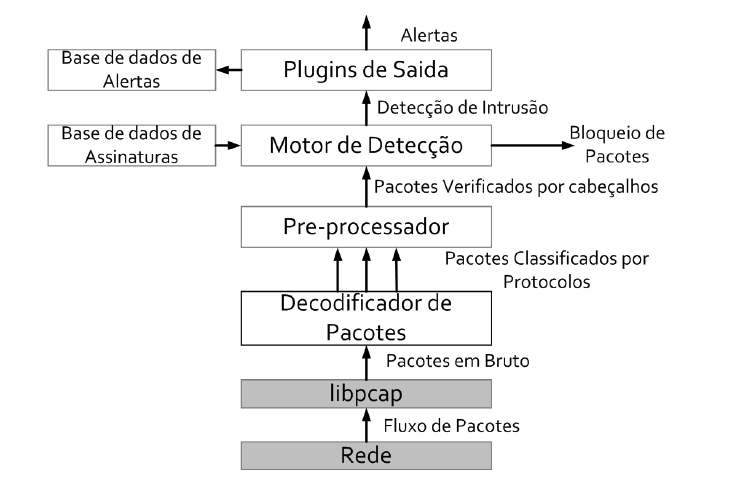
\includegraphics[scale=0.5]{arquitetura-snort.png}
  \legend{Fonte: \cite{arquitetura:martin}}
\end{figure}

O pré-processador, o motor de detecção e os componentes de alerta do Snort são todos \textit{plugins}. Os \textit{Plugins} são programas escritos em conformidade com a API de \textit{plugins} do Snort. Esses programas são usados no core do Snort, mas eles são separados para que as modificações feitas no \textit{core} sejam mais confiáveis e mais fáceis de realizar \cite{snort:andrew}.

O \textit{sniffer} é um dispositivo (\textit{software} ou \textit{hardware}) usado para ver o trafego passante em algum segmento de rede. No caso da Internet, consiste geralmente de trafico IP (composto por diferentes protocolos de alto nível como, TCP, UDP, ICMP, protocolos de roteamento e IPSec). Os pacotes são analisado, interpretados e exibidos de uma forma legível para os humanos.

Um \textit{sniffer} tem os seguintes usos:

\begin{alineas}
\item Analisador de rede e resolução de problemas;
\item Analisador de performance e avaliação comparativa;
\item Capturar senhas em texto plano e outros dados sensíveis.
\end{alineas}

Assim como qualquer outra ferramenta de rede, os \textit{sniffers} podem ser usados tanto para o bem quanto para o mal. Então, criptografar o trafego de rede previne que pessoas sejam capazes de lerem os pacotes capturados \cite{snort:andrew}.

O pré-processador pega o pacote bruto e faz uma checagem utilizando um determinado \textit{plugin}. Esses \textit{plugins} verificam se o pacote tem um tipo particular de comportamento, uma vez determinado, o pacote é enviado para o motor de detecção caso contrário é descartado.

A \autoref{fig_snort_preprocessor}, apresenta como o pré-processador utiliza \textit{plugins} para checar pacotes. O Snort suporta muitos tipos de pré-processadores, cobrindo vários protocolos comumente usados como, IP \textit{fragmentation handling}, \textit{port scanning} e controle de fluxo.

\begin{figure}[htb]
  \centering
  \caption{Uso de \textit{plugins} no pré-processador} \label{fig_snort_preprocessor}
  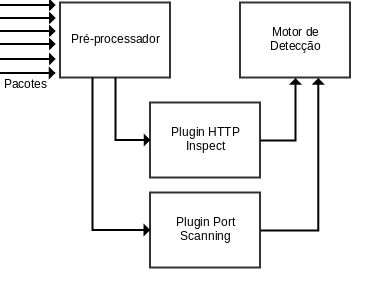
\includegraphics[scale=0.7]{snort_preprocessor.png}
  \legend{Fonte: Autoria própria}
\end{figure}

O uso de \textit{plugins} é uma característica muito útil para o IDS, pois os \textit{plugins} podem ser ativados e desativadas a medida do necessário, otimizando a utilização dos recursos computacionais e geração de alertas \cite{snort:andrew}.

Os pacotes, após passarem por todos os pré-processador, são entregues para o motor de detecção. O motor de detecção recebe esses dados e faz uma checagem utilizando uma base de regras pré-configurado pelo administrador. Se a regra for compatível com os dados do pacote, eles são enviado para o processador de alertas, caso contrário, são descartados \cite{snort:andrew}.

Na \autoref{fig_snort_detecção}, temos os pacotes saindo dos pré-processadores e chegando no motor de detecção. No motor de detecção há uma base de regras configurada, os pacotes são comparados com as assinaturas da base, se coincidirem, uma ação é tomada, caso contrário, o pacote é descartado.

\begin{figure}[!htb]
  \centering
  \caption{Motor de Detecção do Snort} \label{fig_snort_detecção}
  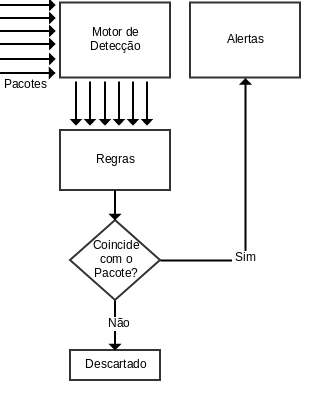
\includegraphics[scale=0.7]{snort_detection.png}
  \legend{Fonte: Autoria própria}
\end{figure}

A base de regras é um conjunto de assinaturas de ataques conhecidos e catalogados. As regras são escritas em formato texto em uma única linha e constituídas por duas partes: 

\begin{alineas}
\item \textbf{Cabeçalho}: São definidos que ações serão tomadas, tipo de pacote (TCP, UDP, ICMP, etc), o IP de origem e destino e suas respectivas portas;
\item \textbf{Opções}: É o conteúdo do pacote que faz ele ser compatível com a regra.
\end{alineas}

Dentre as ações que podem ser tomadas temos:

\begin{alineas}
\item \textbf{\textit{Activation}}: Alerta e chama regra do tipo \textit{dynamic};
\item \textbf{\textit{Dynamic}}: permanece inativa até ser ativado por uma regra \textit{activate}, registrando o tráfego;
\item \textbf{\textit{Alert}}: Gera um alerta usando um método selecionado e então registra os pacotes e dados;
\item \textbf{\textit{Pass}}: Ignora os pacotes;
\item \textbf{\textit{Drop}}: Descarta o pacote (quando configurado para atuar de forma ativa (IPS)); 
\item \textbf{\textit{Log}}: Registra e não alerta.
\end{alineas}

Abaixo temos um exemplo de regra.

\begin{lstlisting}[frame=single]
    alert icmp any any -> any any (msg:"Ping suspeito"; 
    sid:1; resp:icmp_all;)
\end{lstlisting}

Com a regra acima, o Snort gerará um alerta de qualquer pacotes ICMP que estiver passando de qualquer máquina e porta origem (\textbf{any any}) para qualquer máquina e porta destino (\textbf{any any}) e enviará pacotes ICMP para a máquina de origem com as mensagens \textit{host unreachable; network unreachable}.

Se um dado for compatível com uma regra é gerado um alerta. Os alertas podem ser enviados para arquivos de \textit{logs}, através da rede, através de \textit{sockets} UNIX ou Windows Popup (SMB). Os alertas também podem ser armazenados em banco de dados SQL como MySQL e Postgres. Existem vários \textit{plugins} para Perl, PHP e servidores Web para exibir os \textit{logs} através de um interface Web \cite{snort:andrew}.

\subsection{Suricata} \label{sec:suricata}

Suricata é um NIDS de código aberto. Sua primeira versão oficial foi lançado em 2010 e foi desenvolvido e atualmente é mantido pela \textit{Open Information Security Foundation} (OISF). A OISF é uma fundação sem fins lucrativos formada por um grupo multinacional de desenvolvedores \cite{suricata}.

Uma característica marcante desse IDS é a utilização de uma tecnologia de processamento \textit{multithread} para ter benefício dos múltiplos núcleos de um computador. Além de utilizar \textit{hardware} de aceleração para ter um melhor desempenho \cite{arquitetura:martin}.

O Suricata utilizada detecção baseada em assinatura e em anomalias. As assinaturas desenhadas para o Snort funcionam no Suricata, podendo ser otimizadas para o uso em seu motor de detecção. As anomalias dos protocolos são fornecidas pelos pré-processadores, e quando implementado no modo ativo, atua na modalidade de prevenção \cite{arquitetura:martin}.

Embora o código do Suricata ser original, os desenvolvedores não hesitam afirmar que a arquitetura foi inspirada no Snort. Na \autoref{fig_arquitetura-suricata} representa a mesma arquitetura do Snort porém com o mecanismo de \textit{multithread} \cite{arquitetura:martin}. 

%Dessa forma não há necessidade de descrever os componentes pois já foram citados na \autoref{sec:snort}.

\begin{figure}[!htb]
  \centering
  \caption{Arquitetura \textit{Multithread} do Suricata} \label{fig_arquitetura-suricata}
  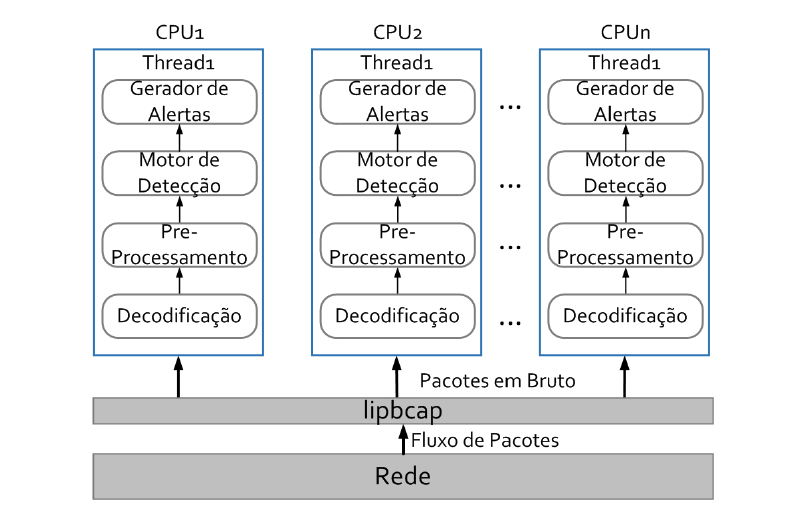
\includegraphics[scale=0.5]{arquitetura-suricata.png} 
  \legend{Fonte: \cite{arquitetura:martin}}
\end{figure}

As assinaturas são de grande importância tanto no Snort quanto no Suricata. Muitas pessoas, por conveniência, utilizam conjunto de regras prontas. As mais usadas são da Emerging Threats (ET) e Talos (anteriormente chamado de VRT) \cite{suricata:rule}. Talos é um grupo de especialistas em segurança de rede trabalhando o tempo todo para descobrir, avaliar e responder de forma proativa as últimas tendências em atividades de \textit{hacking}, tentativa de intrusão, \textit{malware} e vulnerabilidades \cite{snort:talos}. 

A base de assinaturas ET é mantida pela Proofpoint. A Proofpoint é uma empresa especialista em segurança da informação, no site oficial há vários produtos que visam proteger pessoas e dados, detectando e bloqueando ataques e respondendo a essas ameaças \cite{et:proofpoint}.

O fato de existir equipes dedicadas para o desenvolvimento de uma base de regras, torna o uso dessas bases confiáveis, menos custoso, tem termos de tempo, recursos financeiros e de pessoal e fácil implementação. 

\section{Conclusão} \label{sec:idps-conclusao}

Este capítulo apresentou definições sobre IDPS e seus componentes, os tipos existentes e a forma de detecção utilizada. Também foi descrito as ferramentas avaliadas nesse trabalho (Snort e Suricata), destacando suas diferenças e arquiteturas.
